\section{Auto encoders}

The compression and decompression function are learned automatically from unlabeled data rather than hand-engineered by a human. The AE can be used in many different applications, including the generation of SDRs. 

In order for the AE to be a good compression algorithm, we must prevent the network from learning simple solutions. This is achieved by adding a restricted hidden layer (see figure \ref{fig:AE}). By introducing an information bottleneck in the middle of the network, we can prevent the network from learning simple mappings, and force it 
How is the AE useful then? We  And it is, if we allow the network to learn simple mappings. An AE is designed is such a way that makes the copying task difficult by introducing an information bottleneck in the middle of the network. This information bottleneck corresponds to the hidden layer where 
The core idea of an AE is quite simple, but with small tweaks to the architecture and training procedure, the AE can be repurposed. The original purpose of the AE is data compression. Some of the additional use cases of the AE are: remove noise from patterns, reduce the dimensionality of data for visualization purposes (similar to PCA), or generate sparse patterns.

\begin{figure}[h]
    \centering
    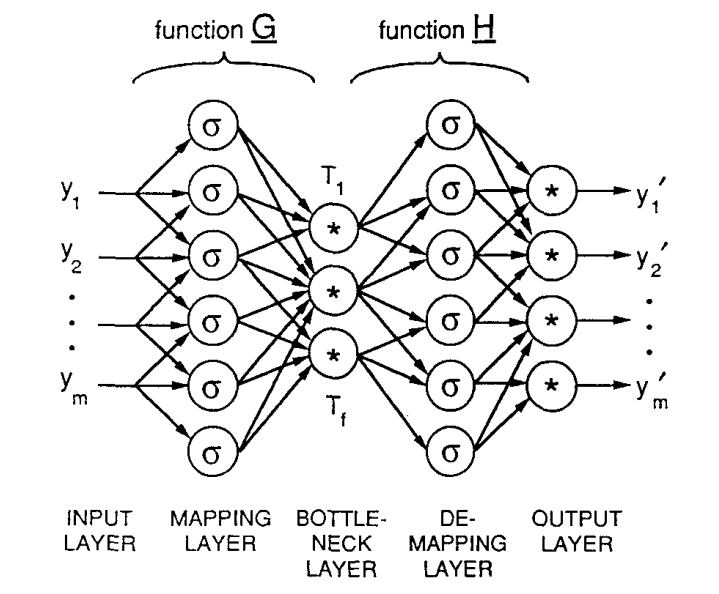
\includegraphics[width=0.9\textwidth]{img/AE.PNG}
    \caption{Architecture of a simple Autoencoder. Adapted from \cite{kramer1991nonlinear}.}
\label{fig:AE}
\end{figure}

The architecture of a simple AE can be seen in figure \ref{fig:AE}.
In general terms, an AE is composed by an encoding function ($h=f(x)$), a decoding function ($r=g(h)$), and a loss function that measures the distance between the coded and decoded representations ($d = L(x,d)$). The encoding and decoding functions are implemented with feed-forward neural networks. These networks can either be trained with back-propagation, or the more biologically plausible recirculation algorithm \cite{hinton1988learning}.
In any case, the interesting thing about AEs is that they measure their training accuracy by comparing how similar the original input is to the reconstructed pattern. Meaning that when a good accuracy is achieved, we have found an accurate compress and decompress information.

The way that AEs learn informative representations is by having a hidden layer $h$ that acts as an information bottleneck (for example by having a small number of units). The hidden layer will make it impossible for the AE to perfectly copy the input. The limited information capacity of the hidden layer will force the network to encode only the most important features of the training examples. If the selected features are relevant, the AE will be able to produce a good reconstruction.

An AE is only useful if the hidden layer has significantly less information capacity than the input/output layer. If the hidden layer was identical to the input/output layer, the AE would be learning the identity function which is completely useless. Regarding the sizes of the original patterns and the new representations, an AE can be classified as:
\begin{itemize}
    \item \textbf{Undercomplete} if the new representation is smaller than the original pattern.
    \item \textbf{Overcomplete} if the new representation is larger than the original pattern.
\end{itemize}
Having a new representation with a different size

If built correctly, the AE will produce informative representation by implicitly performing feature extraction. Additionally, the designer of an AE can tweak the properties of the hidden representation (such as size and sparsity) and thus be able to use the AE as a way to generate SDRs.

section{Biologically plausible representations}
Representing human knowledge on a computer has proven to be a difficult task. The problem stems from the fact that our knowledge of the world is not well-organized. Every rule has exceptions and every fact links to numerous others. This level of complexity is not well-suited for traditional computer data-structures. In contrast, our brains seem to deal with this complicated knowledge with ease. Our brains do not use dense representations like those used in computers. Instead, they represent knowledge with the sparse activation of its billions of neurons. The brain uses SDRs to encode knowledge \cite{Hawkins-et-al-2016-Book}. One might ask: If real-world data, like images, is dense, how can the brain use SDRs? Indeed, sensory data is not naturally found in the form of SDRs. But we know that our brain has lower functional regions that process the inputs from the senses and generate sparse and distributed activation of neurons in the neocortex. For instance, the visual area of the brain is divided into several hierarchical regions: V1, V2, V4, and IT. The V1 area of the brain is responsible for detecting low-level visual features such as edges, and basic color. The detection of such features results in the activation of a collection of neurons that forms a signal. This signal is passed onto the V2 area which will apply a similar process. After passing through all the regions, the final result will be an SDR that represents what we are sensing \cite{hawkins2004intelligence}. Another example is auditory perception. The sounds that we hear are captured in the cochlea. The cochlea is an organ that has several receptors for different frequencies. A particular sound will result in the sparse activation of the receptors which will result in an SDR.

All-in-all there is a biological analogy between SDR encoders used for Associative memories and biological organs that transform sensory data into sparse neuron activity in biological memories.